\documentclass[11pt]{article}

%--------------------------------------------------
% Packages
%--------------------------------------------------
\usepackage[margin=1in]{geometry}
\usepackage{amsmath,amssymb}
\usepackage{graphicx}
\usepackage{hyperref}
\usepackage{booktabs}
\usepackage{enumitem}
\usepackage{xcolor}
\usepackage{titlesec}
\usepackage{tikz}
\usetikzlibrary{shapes.geometric, arrows.meta, positioning, fit, backgrounds}
\usepackage{fancyhdr}
\usepackage{microtype}
\usepackage{parskip}
\usepackage{tcolorbox}
\tcbuselibrary{skins, breakable}

%--------------------------------------------------
% Colors
%--------------------------------------------------
\definecolor{primary}{RGB}{0,74,148}
\definecolor{accent}{RGB}{220,50,47}
\definecolor{lightgray}{RGB}{245,245,245}
\definecolor{darkgray}{RGB}{80,80,80}
\definecolor{plannerblue}{RGB}{173,216,230}
\definecolor{toolgreen}{RGB}{144,238,144}
\definecolor{llmpurple}{RGB}{216,191,216}
\definecolor{memoryorange}{RGB}{255,228,181}

%--------------------------------------------------
% Section formatting
%--------------------------------------------------
\titleformat{\section}{\large\bfseries\color{primary}}{}{0em}{}[\vspace{-0.5em}\rule{\linewidth}{0.4pt}]
\titleformat{\subsection}{\normalsize\bfseries\color{darkgray}}{}{0em}{}

%--------------------------------------------------
% Header / Footer
%--------------------------------------------------
\pagestyle{fancy}
\fancyhf{}
\rhead{\small\color{darkgray} ESE 561 --- Final Project Proposal}
\lhead{\small\color{darkgray} SAGE: Self-Adaptive Goal-directed Executor}
\cfoot{\thepage}
\renewcommand{\headrulewidth}{0.4pt}

%--------------------------------------------------
% Hyperref setup
%--------------------------------------------------
\hypersetup{
  colorlinks=true,
  linkcolor=primary,
  urlcolor=primary,
  citecolor=primary
}

%--------------------------------------------------
% TColorBox styles
%--------------------------------------------------
\tcbset{
  boxstyle/.style={
    enhanced, breakable,
    colback=lightgray,
    colframe=primary,
    fonttitle=\bfseries,
    boxrule=0.6pt,
    arc=3pt,
    left=6pt, right=6pt, top=4pt, bottom=4pt
  }
}

%==================================================
\begin{document}
%==================================================

%--------------------------------------------------
% Title block
%--------------------------------------------------
\begin{center}
  {\LARGE\bfseries\color{primary} SAGE: Self-Adaptive Goal-directed Executor}\\[4pt]
  {\large A Multi-Tool LLM Agent with Hierarchical Planning\\
  and Evidence-Guided Reasoning}\\[10pt]
  \rule{\linewidth}{1pt}\\[6pt]
  {\normalsize
  \textbf{Course:} ESE 561 --- Artificial Intelligence \hspace{1.5cm}
  \textbf{Proposal Due:} April 12, 2026 \\[4pt]
  \textbf{Team Members:} Shams Rupak \quad $\cdot$ \quad Gagan Sapkota \\[4pt]
  \textbf{Stony Brook University} \hspace{1.8cm} \textbf{Team Size:} 2 (increased complexity)
  }\\[4pt]
  \rule{\linewidth}{0.4pt}
\end{center}

\vspace{0.4em}

%--------------------------------------------------
\section{Motivation and Problem Statement}
%--------------------------------------------------

Large language models have demonstrated remarkable capability in isolated reasoning tasks,
yet they remain fundamentally reactive: given a prompt, they produce an output. This
single-call paradigm collapses under complex, multi-faceted queries that require sustained
goal-directed behavior, tool interaction, self-correction, and adaptive re-planning.

Consider the task: \textit{``Analyze the trade-offs between transformer-based and recurrent
architectures for long-context reasoning, citing empirical evidence and identifying open
research questions.''} A single LLM call yields a plausible but unverifiable response.
A proper answer requires decomposing the question into sub-goals, actively searching for
evidence, evaluating source reliability, reconciling contradictions across sources, and
synthesizing findings with tracked provenance.

\textbf{SAGE} (Self-Adaptive Goal-directed Executor) is designed to tackle exactly this
class of problem. The agent performs \emph{deep research synthesis}: given a complex
research query, it autonomously plans a multi-step investigation, gathers evidence from
external tools, evaluates and critiques that evidence, and produces a structured,
citation-aware synthesis. Crucially, the \emph{planning and decision-making logic resides
in the agent layer}, not inside the LLM, making the system transparent, auditable, and
correctable.

This project is motivated by a central question that runs through the course:
\textit{Where does the intelligence of an LLM-based system come from---the neural model,
or the surrounding structure?} SAGE is designed to make that boundary explicit and
empirically interrogable. By implementing all planning logic as deterministic Python code and scoping the LLM strictly to per-step reasoning, we can measure the contribution of each layer through a controlled ablation study.

%--------------------------------------------------
\section{Project Topic and Scope}
%--------------------------------------------------

\textbf{Domain:} Automated research question decomposition, multi-source evidence
gathering, and synthesis into a structured analytical report.

\textbf{Input:} A complex, open-ended research or analytical question (e.g., from
science, technology policy, or comparative systems analysis).

\textbf{Output:} A structured synthesis document containing: a hierarchical answer with
sub-question responses, source provenance, confidence scores per claim, identified
contradictions, and a gap analysis with suggested follow-up directions.

\textbf{Scope for a two-person team:}
\begin{itemize}[leftmargin=1.5em, itemsep=2pt]
  \item Full agent loop implementation in Python (5 tools, 3-stage planning pipeline)
  \item Empirical evaluation across $\geq$5 diverse research queries
  \item Ablation study comparing three conditions: full SAGE agent with planner vs.\ flat ReAct baseline (no planner, no critic) vs.\ single LLM call baseline (no tools, no planning)
  \item Final report analyzing where planning helps and where LLM capability dominates, including a dedicated failure analysis section
\end{itemize}

%--------------------------------------------------
\section{High-Level Agent Architecture}
%--------------------------------------------------

SAGE decomposes the agent into five explicit layers, as shown in Figure~\ref{fig:arch}.
Each layer has a defined interface, ensuring that planning logic and LLM reasoning remain
clearly separated. The five layers are: (1)~a deterministic Hierarchical Planner that decomposes queries into a DAG of sub-goals and schedules their execution, (2)~an LLM Reasoning Engine that proposes tool calls within individual sub-goals via a ReAct-style loop, (3)~a Tool Execution Layer providing five callable tools, (4)~an Evidence Critic that evaluates evidence quality and emits control signals, and (5)~a shared State and Memory module that enables cross-step coherence.

\begin{figure}[h!]
\centering
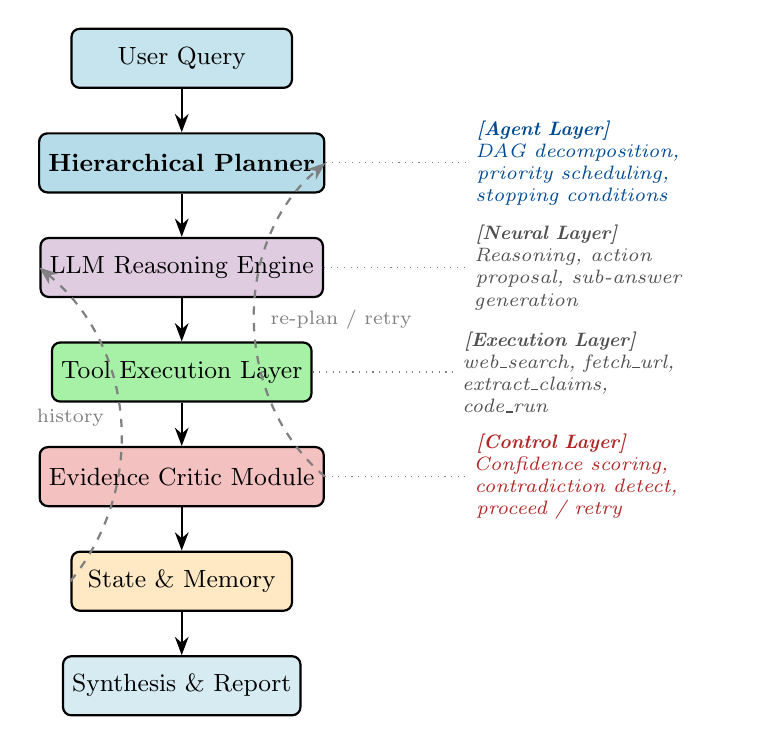
\begin{tikzpicture}[
  node distance=0.55cm and 0.4cm,
  every node/.style={font=\small},
  block/.style={rectangle, rounded corners=3pt, minimum width=2.8cm,
                minimum height=0.75cm, text centered, draw, thick},
  arrow/.style={-Stealth, thick},
  dasharrow/.style={-Stealth, thick, dashed, color=gray}
]

%--- Layers (left column labels) ---%
\node[block, fill=plannerblue!70]  (input)    {User Query};
\node[block, fill=plannerblue!90,  below=of input]  (planner)  {\textbf{Hierarchical Planner}};
\node[block, fill=llmpurple!80,    below=of planner] (llm)     {LLM Reasoning Engine};
\node[block, fill=toolgreen!80,    below=of llm]    (tools)    {Tool Execution Layer};
\node[block, fill=accent!30,       below=of tools]  (critic)   {Evidence Critic Module};
\node[block, fill=memoryorange!80, below=of critic] (memory)   {State \& Memory};
\node[block, fill=plannerblue!50,  below=of memory] (synth)    {Synthesis \& Report};

%--- Arrows (main flow) ---%
\draw[arrow] (input)   -- (planner);
\draw[arrow] (planner) -- (llm);
\draw[arrow] (llm)     -- (tools);
\draw[arrow] (tools)   -- (critic);
\draw[arrow] (critic)  -- (memory);
\draw[arrow] (memory)  -- (synth);

%--- Feedback arrows ---%
\draw[dasharrow] (critic.east)  to[bend left=50]
  node[right, xshift=2pt, font=\scriptsize, color=gray]{re-plan / retry}
  (planner.east);
\draw[dasharrow] (memory.west)  to[bend right=45]
  node[left, xshift=-2pt, font=\scriptsize, color=gray]{history}
  (llm.west);

%--- Right-side annotation ---%
\node[right=1.8cm of planner, font=\scriptsize\itshape, color=primary,
      text width=3.2cm, align=left]
  (ann1) {\textbf{[Agent Layer]}\\ DAG decomposition,\\ priority scheduling,\\ stopping conditions};

\node[right=1.8cm of llm, font=\scriptsize\itshape, color=darkgray,
      text width=3.2cm, align=left]
  (ann2) {\textbf{[Neural Layer]}\\ Reasoning, action\\ proposal, sub-answer\\ generation};

\node[right=1.8cm of tools, font=\scriptsize\itshape, color=darkgray,
      text width=3.2cm, align=left]
  (ann3) {\textbf{[Execution Layer]}\\ web\_search, fetch\_url,\\ extract\_claims,\\ code\_run};

\node[right=1.8cm of critic, font=\scriptsize\itshape, color=accent!80!black,
      text width=3.2cm, align=left]
  (ann4) {\textbf{[Control Layer]}\\ Confidence scoring,\\ contradiction detect,\\ proceed / retry};

\draw[dotted, gray] (planner.east) -- (ann1.west);
\draw[dotted, gray] (llm.east)    -- (ann2.west);
\draw[dotted, gray] (tools.east)  -- (ann3.west);
\draw[dotted, gray] (critic.east) -- (ann4.west);

\end{tikzpicture}
\caption{SAGE architecture. \textbf{Blue}: planner-controlled logic. \textbf{Purple}:
LLM reasoning. \textbf{Green}: tool execution. \textbf{Red}: evidence evaluation.
\textbf{Orange}: shared memory. Dashed arrows indicate feedback/re-planning paths.}
\label{fig:arch}
\end{figure}

\subsection{Layer Descriptions}

\textbf{(1) Hierarchical Planner (Agent Layer).}
The planner is a deterministic Python module---not an LLM---that receives the user query
and produces a Directed Acyclic Graph (DAG) of sub-goals. Each node in the DAG
represents an atomic sub-question with explicit prerequisites (edges). The planner
maintains a priority queue ordered by dependency depth and estimated information gain.
This is the primary site of explicit decision-making in SAGE. The planner consists of three sub-modules: a \emph{Decomposer} that generates and validates sub-questions, a \emph{Scheduler} that determines execution order via a min-heap priority queue, and a \emph{Re-planner} that inserts new sub-goals when the Critic escalates.

\textbf{(2) LLM Reasoning Engine.}
Within each sub-goal, the LLM is invoked in a ReAct-style loop: it receives the
sub-question, tool descriptions, and the current observation history, and it proposes
either a tool call or a direct reasoning step. The LLM does \emph{not} decide the
overall execution order---that is the planner's role. The ReAct loop runs for a maximum of 5 steps per sub-goal, producing structured \texttt{Thought $\to$ Action $\to$ Observation} triples that form the reasoning trace.

\textbf{(3) Tool Execution Layer.}
A suite of five stateless tools callable by the agent, each returning a standardized result dictionary \texttt{\{success: bool, content: str, metadata: dict\}}:
\begin{itemize}[leftmargin=1.5em, itemsep=1pt]
  \item \texttt{web\_search(query)} --- retrieves ranked snippets via Tavily API
  \item \texttt{fetch\_url(url)} --- fetches and parses full page content via \texttt{httpx} + BeautifulSoup
  \item \texttt{extract\_claims(text)} --- LLM-powered structured claim extraction with confidence scores
  \item \texttt{code\_run(snippet)} --- Python execution sandbox with timeout guard
  \item \texttt{cross\_reference(claim\_list)} --- checks internal consistency across claims
\end{itemize}

\textbf{(4) Evidence Critic Module.}
After each sub-goal resolves, the Critic---a separate, structured LLM call with a fixed
JSON schema---assigns a confidence score $c \in [0,1]$, flags contradictions with prior
evidence, and emits one of three control signals: \texttt{ACCEPT}, \texttt{RETRY} (with
revised query), or \texttt{ESCALATE} (trigger re-plan). Crucially, the Critic's LLM output is subject to deterministic override rules: if max retries are exhausted, \texttt{RETRY} is overridden to \texttt{ESCALATE}; if confidence exceeds the threshold, the signal is overridden to \texttt{ACCEPT}. These overrides ensure the agent loop always terminates. This is the key feedback
mechanism that makes SAGE self-correcting.

\textbf{(5) State \& Memory.}
A structured \texttt{AgentState} object stores: the current DAG state, per-node evidence and confidence
scores, the full reasoning trace (thoughts, tool calls, observations), and a provenance
map linking each claim to its source URL. This shared memory is passed into every LLM call,
enabling cross-step coherence without requiring the LLM to re-derive prior findings.

%--------------------------------------------------
\section{Planning Component}
%--------------------------------------------------

\begin{tcolorbox}[boxstyle, title={Core Planning Design}]
The planning logic in SAGE is architecturally \emph{external to the LLM}. The LLM
proposes actions within a sub-goal; the agent determines what sub-goals exist, in what
order they execute, and what to do when evidence is insufficient.
\end{tcolorbox}

\subsection{Where Planning Is Introduced}

\begin{enumerate}[leftmargin=1.5em, label=\textbf{\arabic{enumi}.}, itemsep=4pt]

  \item \textbf{Query Decomposition (Plan-and-Execute).}
  Before any tool-using LLM call, the planner performs \emph{hierarchical decomposition}: the root
  query is broken into 3--6 sub-goals. The decomposition uses a heuristic ruleset (e.g., detect conjunctions,
  comparative structures, causal chains) to estimate query complexity, followed by a single LLM call to generate
  an initial sub-question list. The planner then \emph{validates} these proposals deterministically: it checks for valid JSON structure, removes hallucinated dependency references, deduplicates, detects cycles, and constructs the DAG. If the LLM's response is malformed, the planner falls back to a single-node DAG containing the original query. The key design insight is that the LLM \emph{suggests} but the planner \emph{decides}.

  \item \textbf{Priority Scheduling (Action Selection).}
  The planner maintains a min-heap priority queue over DAG nodes. Priority is a weighted function
  of three factors: dependency depth (nodes with no unresolved prerequisites are eligible first), estimated
  relevance (cosine similarity of the sub-question embedding to the root query, computed via \texttt{sentence-transformers}), and current confidence deficit (low-confidence nodes are re-prioritized after retries). The composite priority score is:
  \[
  \text{priority} = w_d \cdot \frac{\text{depth}}{\max(\text{depth})} + w_r \cdot (1 - \text{relevance}) + w_c \cdot (1 - \text{confidence})
  \]
  where $w_d = 0.4$, $w_r = 0.3$, $w_c = 0.3$. This is
  implemented entirely in Python with no LLM involvement.

  \item \textbf{Stopping Conditions (Termination Logic).}
  The agent loop terminates when: (a) all DAG nodes have $c \geq \tau$ (confidence
  threshold, default $\tau=0.75$), (b) the maximum iteration count is reached, or (c)
  no more nodes are eligible for execution. These conditions prevent both premature termination and infinite loops.

  \item \textbf{Re-planning on Failure (Adaptive Control).}
  When the Critic emits \texttt{ESCALATE}, the re-planner inserts 1--3 new sub-goals into the
  DAG to address identified gaps. The failed node is marked as \texttt{FAILED}, and new nodes inherit its dependency edges. This is analogous to plan repair in classical AI and enables
  SAGE to adapt its strategy mid-execution without discarding prior evidence.

  \item \textbf{Synthesis Ordering (Structured Aggregation).}
  The final synthesis step is driven by a topological sort of the DAG (Kahn's algorithm), ensuring that
  dependent claims are always synthesized after their prerequisites. This structural
  property guarantees logical coherence in the output, independent of LLM output quality.

\end{enumerate}

%--------------------------------------------------
\section{Agent Design Patterns Used}
%--------------------------------------------------

SAGE incorporates three complementary design patterns from the course material:

\begin{center}
\begin{tabular}{@{}lll@{}}
\toprule
\textbf{Pattern} & \textbf{Where Applied} & \textbf{Purpose} \\
\midrule
Plan-and-Execute & DAG planner $\to$ sub-goal execution & Separate strategy from tactics \\
ReAct Loop       & Per sub-goal inner loop              & Ground reasoning in tool observations \\
Self-Reflection  & Evidence Critic module               & Detect and correct low-quality evidence \\
\bottomrule
\end{tabular}
\end{center}

The combination of all three is a deliberate design choice: Plan-and-Execute alone
produces brittle agents that cannot recover from mid-plan failures; ReAct alone lacks
global coherence; Self-Reflection alone without structure produces circular reasoning.
SAGE's contribution is the explicit integration of all three with clean architectural
boundaries, enabling us to measure each layer's contribution through ablation.

%--------------------------------------------------
\section{Technical Stack and Division of Work}
%--------------------------------------------------

\begin{center}
\begin{tabular}{@{}ll@{}}
\toprule
\textbf{Component} & \textbf{Technology} \\
\midrule
LLM backend & Groq API (\texttt{llama-3.3-70b-versatile}) --- free tier \\
Fallback LLM & Google Gemini 1.5 Flash --- free tier \\
Web search tool & Tavily API (free tier, agent-optimized) \\
URL fetcher & \texttt{httpx} + BeautifulSoup \\
Code execution sandbox & \texttt{subprocess} with timeout guard \\
Claim extraction & Structured LLM call with JSON schema \\
State management & Pure Python (\texttt{dataclasses}, \texttt{heapq}) \\
Embedding / similarity & \texttt{sentence-transformers} (\texttt{all-MiniLM-L6-v2}) \\
Terminal output & \texttt{rich} library \\
Testing & \texttt{pytest} \\
Evaluation & Manual rubric + structural quality scoring \\
\bottomrule
\end{tabular}
\end{center}

No external agent frameworks (LangChain, AutoGPT, CrewAI, etc.) are used. The entire agent structure is implemented from scratch to ensure full understanding and to satisfy the course requirement that planning be an explicit, auditable part of the system.

\textbf{Division of work:}
\begin{itemize}[leftmargin=1.5em, itemsep=2pt]
  \item \textit{Shams Rupak}: Hierarchical Planner module (DAG data structure, decomposer, priority scheduler, re-planner), ablation study design, evaluation framework, final report.
  \item \textit{Gagan Sapkota}: Tool layer implementation (5 tools + registry), Evidence Critic module,
        state/memory management, synthesis pipeline, demo interface.
\end{itemize}

%--------------------------------------------------
\section{Connection to Course Themes}
%--------------------------------------------------

SAGE is designed as a living case study for the four modules of ESE 561:

\begin{itemize}[leftmargin=1.5em, itemsep=3pt]
  \item \textbf{Module 1 (Search \& Planning):} The DAG planner and priority scheduler
        directly instantiate classical planning concepts---state representation, action
        selection, and goal decomposition---in an LLM context. The scheduler's priority function echoes informed search strategies, and the re-planner implements plan repair.
  \item \textbf{Module 2 (Neural Models):} The LLM serves as the reasoning and
        representation engine, but its outputs are always \emph{interpreted and validated}
        by the agent layer, making the boundary between neural capability and system structure explicit.
  \item \textbf{Module 3 (Neuro-Symbolic Integration):} SAGE exemplifies the
        neuro-symbolic paradigm: neural generation (LLM) + symbolic structure (DAG,
        rules, schemas). The Critic module enforces logical constraints on LLM outputs through deterministic override rules.
  \item \textbf{Module 4 (Limitations of AI):} The ablation study will directly surface
        failure modes---hallucination, planning horizon limits, tool grounding failures,
        confidence miscalibration---providing empirical grounding for the course's critical AI analysis.
\end{itemize}

%--------------------------------------------------
\section{Expected Outcomes and Evaluation}
%--------------------------------------------------

\textbf{Primary deliverables:}
\begin{enumerate}[leftmargin=1.5em, itemsep=2pt]
  \item Fully working SAGE system runnable end-to-end on $\geq$5 diverse queries
  \item Live demo showing the agent loop, planner decisions, and Critic interventions in rich terminal output
  \item Ablation table: SAGE vs.\ single LLM call vs.\ flat ReAct (no planner), comparing sub-goal count, tool calls, confidence scores, citation count, report structure, and execution time
  \item Final report with architecture analysis, design justification, and a dedicated failure mode analysis section
\end{enumerate}

\textbf{Success criteria:} The system runs reliably across test queries without crashes,
the planner demonstrably changes execution behavior (verified via logs), and the Critic
module triggers at least one re-plan or retry per complex query. Evaluation will
prioritize design clarity and understanding over raw output quality.

\textbf{Evaluation metrics:} We will compare conditions using structural quality metrics: number of sub-goals decomposed, number of tool calls grounded in external sources, average Evidence Critic confidence, number of citations in the final report, and report length/organization. These metrics are more meaningful for research synthesis than automated text similarity scores, as synthesis quality is inherently multi-dimensional.

%--------------------------------------------------
\section*{Summary}
%--------------------------------------------------

\begin{tcolorbox}[boxstyle, title={Project Summary}]
\textbf{Project Name:} SAGE --- Self-Adaptive Goal-directed Executor \\
\textbf{Team:} Shams Rupak, Gagan Sapkota (2 members) \\
\textbf{Task:} Automated research synthesis via multi-tool LLM agent \\
\textbf{Planning Component:} DAG-based hierarchical planner (deterministic Python),
priority scheduler, confidence-gated stopping conditions, adaptive re-planning \\
\textbf{Planning Location:} Agent layer (external to LLM) --- sub-goal decomposition,
execution scheduling, termination logic, re-planning on evidence failure \\
\textbf{Design Patterns:} Plan-and-Execute + ReAct + Self-Reflection \\
\textbf{Key Differentiator:} All high-level decision-making is auditable, code-level
logic; the LLM is scoped strictly to per-step reasoning and tool proposal.
\end{tcolorbox}

\end{document}